\section{Antenna Design 2 -- Triangle-Feed Antenna}
In this section, the results from Section~\ref{sec:techsol_triang} will be repeated, having the phone in read mode, play mode, and talk mode. Additionally, the maximum SAR value, recorded in the users head, will be simulated. The antenna positions, for each use case, are shown in Figure~\ref{fig:triang_positions}.

\begin{figure}[htbp]
    \centering
    \begin{subfigure}[b]{0.24\linewidth}
        \centering
        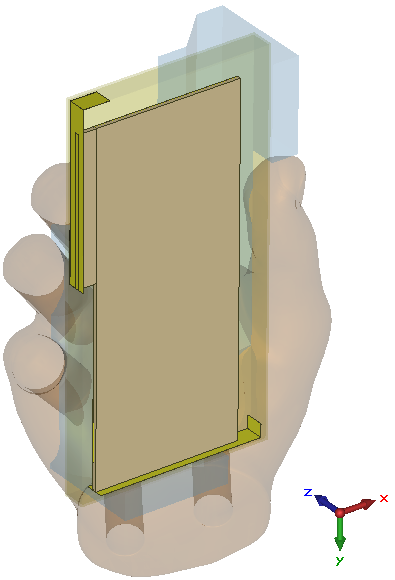
\includegraphics[width=\linewidth,height=4cm,keepaspectratio]{img/tech_sol/trianglefeed/read_mode/3d.PNG}
        \caption{Read mode.}
    \end{subfigure}
    \begin{subfigure}[b]{0.24\linewidth}
        \centering
        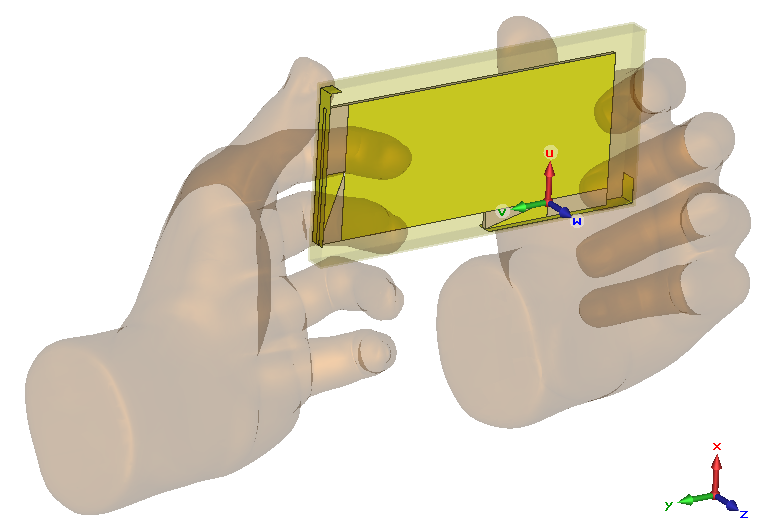
\includegraphics[width=\linewidth,height=4cm,keepaspectratio]{img/tech_sol/trianglefeed/play_mode/3d.PNG}
        \caption{Play mode.}
    \end{subfigure}
    \begin{subfigure}[b]{0.24\linewidth}
        \centering
        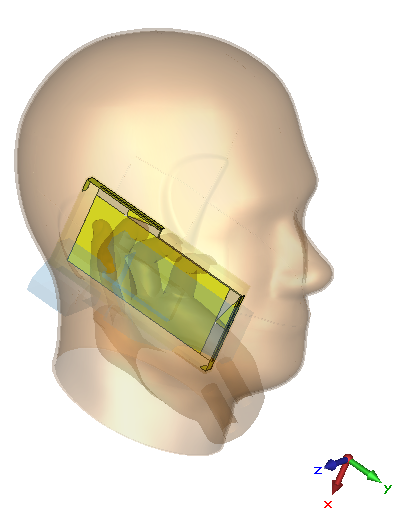
\includegraphics[width=\linewidth,height=4cm,keepaspectratio]{img/tech_sol/trianglefeed/talk_mode/3d.PNG}
        \caption{Talk mode.}
    \end{subfigure}
    \begin{subfigure}[b]{0.24\linewidth}
        \centering
        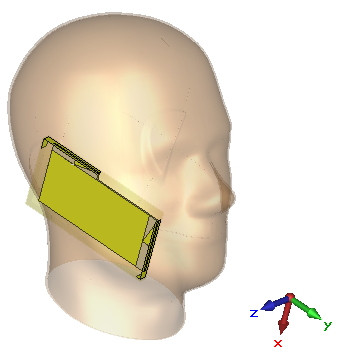
\includegraphics[width=\linewidth,height=4cm,keepaspectratio]{img/tech_sol/trianglefeed/sar/3d.PNG}
        \caption{SAR.}
    \end{subfigure}
    \caption{Antenna position for each user effect simulation.}
    \label{fig:triang_positions}
\end{figure}

\FloatBarrier
\subsection{Read Mode}
The S-parameters with the tunable capacitors set to their minima are shown in Figure~\ref{fig:triang_sparam_read}. It is seen that that the low band of the side antenna has been tuned down to around the middle of the low band. As it is not possible to tune the resonance further upwards, the bands around \SI{960}{MHz} are not covered at greater than \SI{6}{dB} return loss. The high band is still almost covered at around \SI{5}{dB} return loss. The top antenna, on the other hand, almost covers both the low and the high band simultaneously.

The S-parameters, when sweeping the tunable capacitors, are shown in Figure~\ref{fig:tiang_sparam_sweep_read}. The maximum impedance-bandwidths are summed up in Table~\ref{tab:bw_sol2read}. From this it is again clear that only the top antenna is able to cover the high end of the low band. None of the antennas can cover the high band at \SI{6}{dB} return loss. However, as they can cover the high band at greater than \SI{5}{dB}, this is not considered a problem.

The correlation between the antennas, when sweeping the tunable capacitors, are shown in Figure~\ref{fig:corr_sol2_read}. The correlation is, for frequencies above \SI{750}{MHz}, below 0.5 when sweeping the top antenna. When sweeping the side antenna, the correlation remains below 0.5 for all capacitor settings. The correlation has dropped significantly from the free-space simulation in Figure~\ref{fig:corr_sol2}.

The efficiencies for each antenna, when sweeping the tuning capacitors, are shown in Figure~\ref{fig:eff_sol2read}. It is seen that the efficiency, generally, has decreased from the free space simulation in Chapter~\ref{cha:nousersim}. At  \SI{-3}{dB} efficiency, there is no bandwidth left. At \SI{-6}{dB}, the most of the bands can be covered except at the lower part of the low band for the side antenna where the efficiency decreases to a maximum of \SI{-7}{dB}. The efficiency in the high band is generally higher than in the low band.

\begin{figure}[htbp]
    \centering
    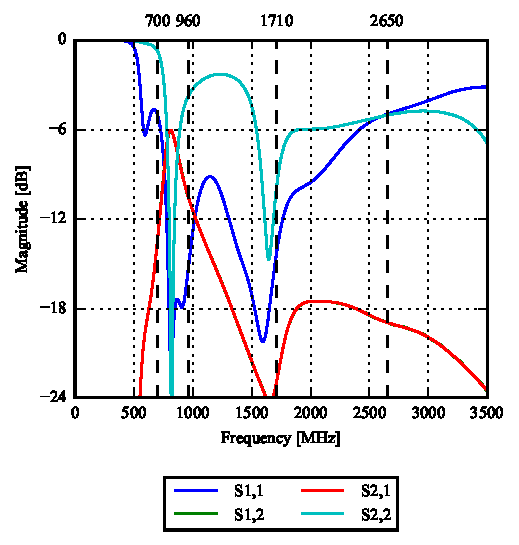
\includegraphics{img/tech_sol/trianglefeed/read_mode/sparams.pdf}
    \caption{Triangular feed antenna in read mode. S-parameters with both tuning capacitors fixed at \SI{0.3}{pF}.}
    \label{fig:triang_sparam_read}
\end{figure}

\begin{table}[htbp]
    \centering
    \begin{tabular}{|l|l|r|r|r|}
        \hline
        Antenna & Band & Start [MHz] & Stop [MHz] & Bandwidth [MHz] \\
        \hline
        Top     & Low  & 570         & 2583       & 2013 \\
        Side    & Low  & 779         & 891        & 112  \\
        \hline
        Top     & High & 570         & 2583       & 2013 \\
        Side    & High & 1506        & 2623       & 1117 \\
        \hline
    \end{tabular}
    \caption{Triangle feed antenna in read mode. Maximum bandwidth obtained in the low and high band for the top and the side antenna, respectively. It is seen that, for the low capacitor settings on the top antenna, both the low and high band are covered at the same time.}
    \label{tab:bw_sol2read}
\end{table}

\begin{figure}[htbp]
   \begin{subfigure}[b]{0.49\linewidth}
        \centering
        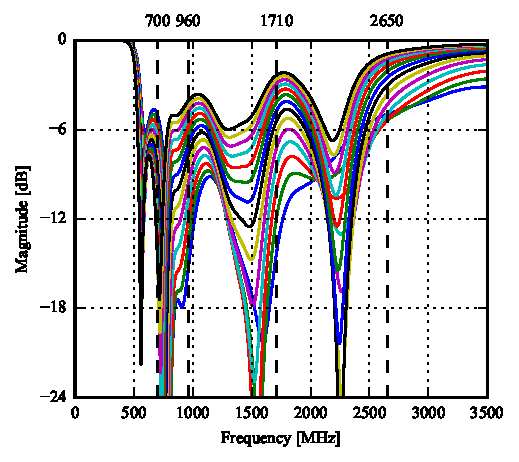
\includegraphics{img/tech_sol/trianglefeed/read_mode/Csh1s11.pdf}
        \caption{$S_{11}$, sweeping $C_1$ and fixing $C_2$.}
    \end{subfigure}
    \hfill
    \begin{subfigure}[b]{0.49\linewidth}
        \centering
        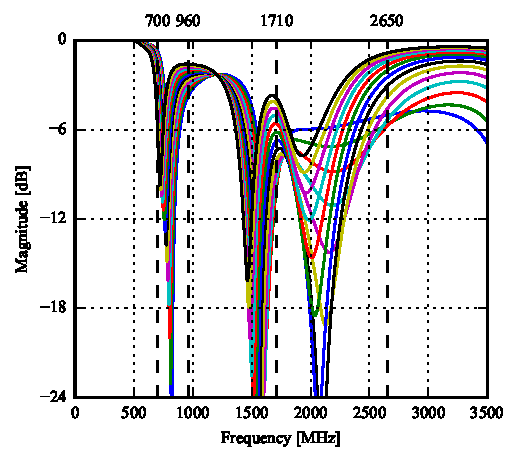
\includegraphics{img/tech_sol/trianglefeed/read_mode/Csh2s22.pdf}
        \caption{$S_{22}$, sweeping $C_1$ and fixing $C_2$.}
    \end{subfigure}
    \\
    \begin{subfigure}[b]{0.49\linewidth}
        \centering
        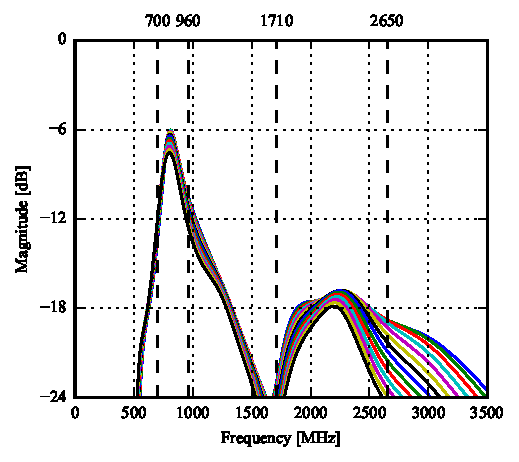
\includegraphics{img/tech_sol/trianglefeed/read_mode/Csh1s21.pdf}
        \caption{$S_{21}$, sweeping $C_1$ and fixing $C_2$.}
    \end{subfigure}
    \hfill
    \begin{subfigure}[b]{0.49\linewidth}
        \centering
        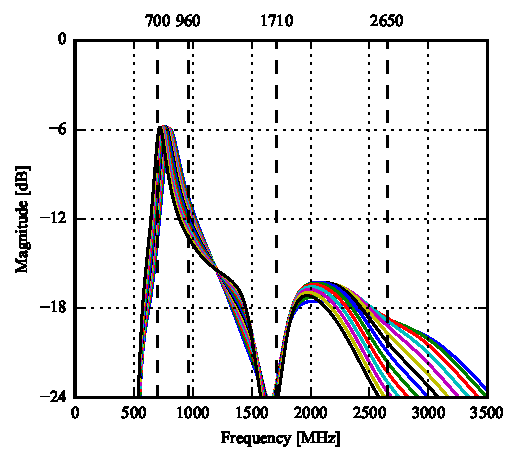
\includegraphics{img/tech_sol/trianglefeed/read_mode/Csh2s21.pdf}
        \caption{$S_{21}$, sweeping $C_2$ and fixing $C_1$.}
    \end{subfigure}
    \caption{Triangle feed antenna in read mode. Parameter sweep for tuning the shunt capacitor of each antenna, $C_1$ and $C_2$ for port 1 and 2, respectively. Port 1 is the top antenna and port 2 is the side antenna.}
    \label{fig:tiang_sparam_sweep_read}
\end{figure}

% Correlation
\begin{figure}[htbp]
    \centering
    \begin{subfigure}{0.49\linewidth}
        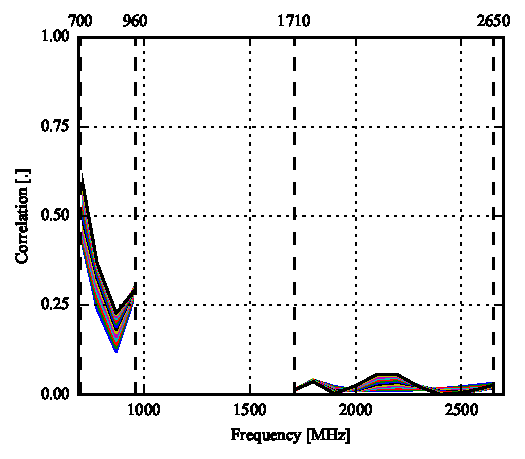
\includegraphics{img/tech_sol/trianglefeed/read_mode/correlation_Csh1-sweep}
        \caption{Sweeping $C_1$ and fixing $C_2$.}
    \end{subfigure}
    \hfill
    \begin{subfigure}{0.49\linewidth}
        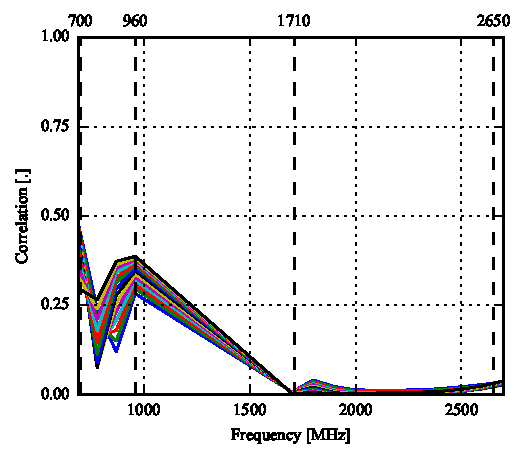
\includegraphics{img/tech_sol/trianglefeed/read_mode/correlation_Csh2-sweep}
        \caption{Sweeping $C_2$ and fixing $C_1$.}
    \end{subfigure}
    \caption{Triangle feed antenna in read mode. Correlation between antennas then sweeping tuning capacitors. Here, $C_1$ and $C_2$ are the tuning capacitor for the top and side antenna, respectively.}
    \label{fig:corr_sol2_read}
\end{figure}

% Efficiency
\begin{figure}[htbp]
    \centering
    \begin{subfigure}{0.49\linewidth}
        \centering
        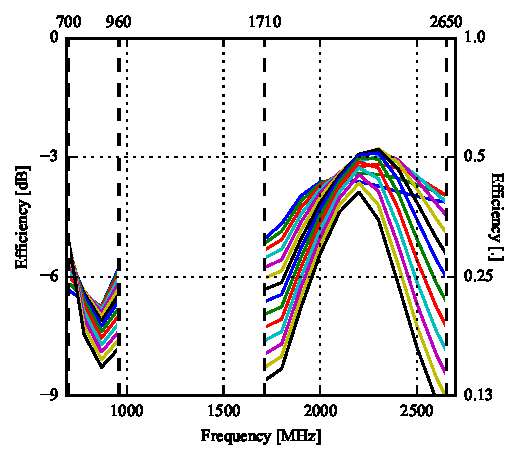
\includegraphics{img/tech_sol/trianglefeed/read_mode/efficiency-ac1-Csh1.pdf}
        \caption{Top antenna. Sweeping $C_1$, fixing $C_2$.}
    \end{subfigure}
    \hfill
    \begin{subfigure}{0.49\linewidth}
        \centering
        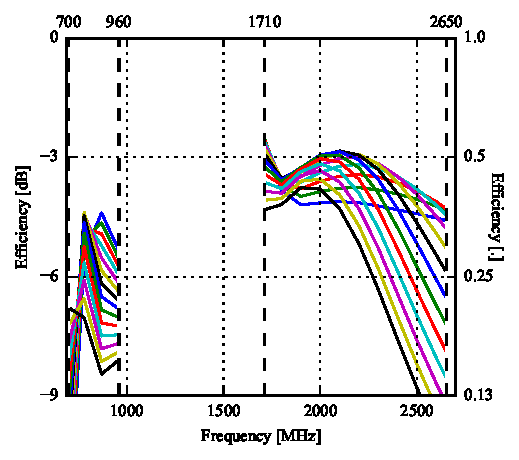
\includegraphics{img/tech_sol/trianglefeed/read_mode/efficiency-ac2-Csh2.pdf}
        \caption{Side antenna. Sweeping $C_2$, fixing $C_1$.}
    \end{subfigure}
    \caption{Triangle feed antenna in read mode. Efficiency for each antenna when sweeping the tuning capacitors. Here, $C_1$ and $C_2$ are the tuning capacitor for the top and side antenna, respectively.}
    \label{fig:eff_sol2read}
\end{figure}


\FloatBarrier
\subsection{Play Mode}

The S-parameters with the tunable capacitors set to their minima are shown in Figure~\ref{fig:triang_sparam_play}. Here, both the top and side antennas have been tuned down. As for read mode, the side antenna can only cover the lower half of the low band whereas the top antenna can cover cover the lower band at greater than \SI{5}{dB} return loss.

The S-parameters, when sweeping the tunable capacitors, are shown in Figure~\ref{fig:tiang_sparam_sweep_play}. The maximum impedance-bandwidths are summed up in Table~\ref{tab:bw_sol2play}. It is seen, that both antennas almost cover the high band. The tunable bandwidth is still large enough to cover the LTE bands in the low band.

The correlation between the antennas, when sweeping the tunable capacitors, are shown in Figure~\ref{fig:corr_sol2_play}. The correlation is similar to that of the read mode.

The efficiencies for each antenna, when sweeping the tuning capacitors, are shown in Figure~\ref{fig:eff_sol2play}. Compared to the read mode, the high band efficiency of the top antenna has decreased more than the low band efficiency. The side antenna is very similar to the read mode results.

\begin{figure}[htbp]
    \centering
    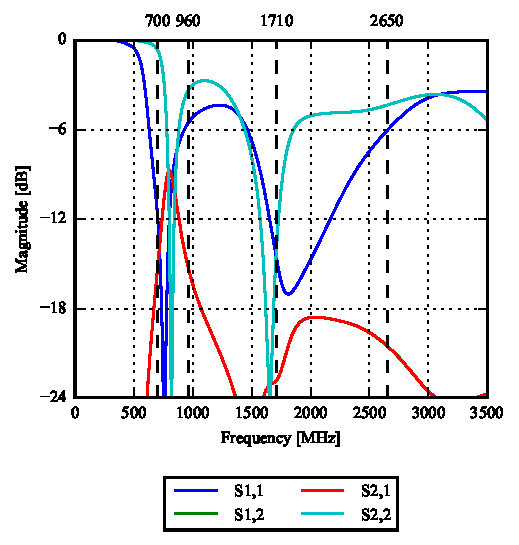
\includegraphics{img/tech_sol/trianglefeed/play_mode/sparams.pdf}
    \caption{Triangular feed antenna in play mode. S-parameters with both tuning capacitors fixed at \SI{0.3}{pF}.}
    \label{fig:triang_sparam_play}
\end{figure}

\begin{table}[htbp]
    \centering
    \begin{tabular}{|l|l|r|r|r|}
        \hline
        Antenna & Band & Start [MHz] & Stop [MHz] & Bandwidth [MHz] \\
        \hline
        Top     & Low  & 629         & 928        & 299  \\
        Side    & Low  & 780         & 881        & 101  \\
        \hline
        Top     & High & 1379        & 2703       & 1324 \\
        Side    & High & 1388        & 2559       & 1171 \\
        \hline
    \end{tabular}
    \caption{Triangle feed antenna in play mode. Maximum bandwidth obtained in the low and high band for the top and the side antenna, respectively. The bandwidth for the side antennas high band is ignoring the slight rise above \SI{-6}{dB} in the middle of the high band.}
    \label{tab:bw_sol2play}
\end{table}

\begin{figure}[htbp]
   \begin{subfigure}[b]{0.49\linewidth}
        \centering
        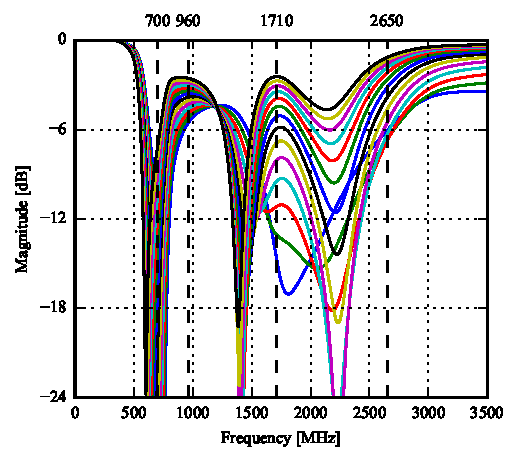
\includegraphics{img/tech_sol/trianglefeed/play_mode/Csh1s11.pdf}
        \caption{$S_{11}$, sweeping $C_1$ and fixing $C_2$.}
    \end{subfigure}
    \hfill
    \begin{subfigure}[b]{0.49\linewidth}
        \centering
        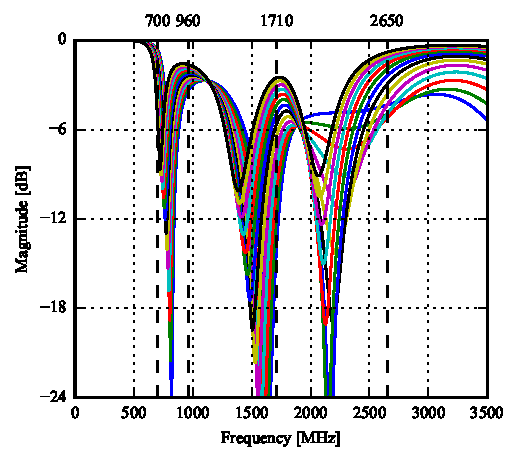
\includegraphics{img/tech_sol/trianglefeed/play_mode/Csh2s22.pdf}
        \caption{$S_{22}$, sweeping $C_1$ and fixing $C_2$.}
    \end{subfigure}
    \\
    \begin{subfigure}[b]{0.49\linewidth}
        \centering
        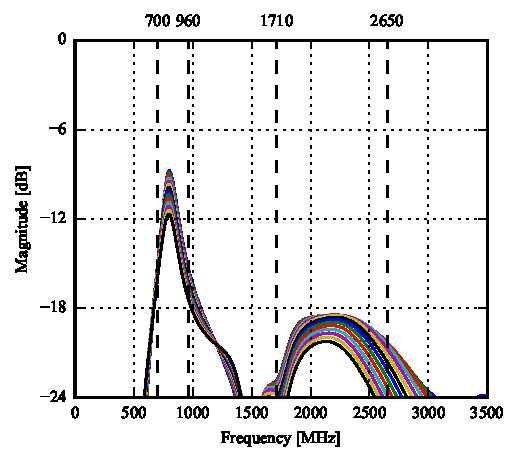
\includegraphics{img/tech_sol/trianglefeed/play_mode/Csh1s21.pdf}
        \caption{$S_{21}$, sweeping $C_1$ and fixing $C_2$.}
    \end{subfigure}
    \hfill
    \begin{subfigure}[b]{0.49\linewidth}
        \centering
        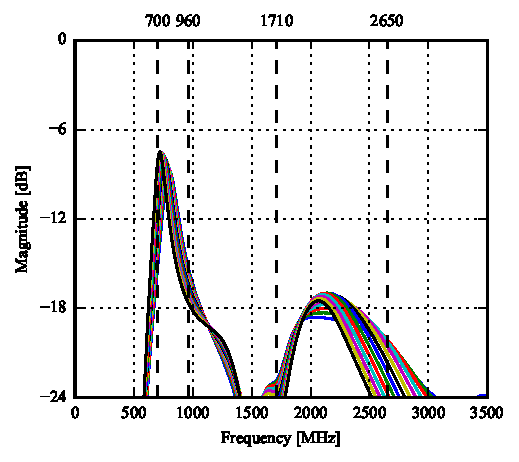
\includegraphics{img/tech_sol/trianglefeed/play_mode/Csh2s21.pdf}
        \caption{$S_{21}$, sweeping $C_2$ and fixing $C_1$.}
    \end{subfigure}
    \caption{Triangle feed antenna in play mode. Parameter sweep for tuning the shunt capacitor of each antenna, $C_1$ and $C_2$ for port 1 and 2, respectively. Port 1 is the top antenna and port 2 is the side antenna.}
    \label{fig:tiang_sparam_sweep_play}
\end{figure}

% Correlation
\begin{figure}[htbp]
    \centering
    \begin{subfigure}{0.49\linewidth}
        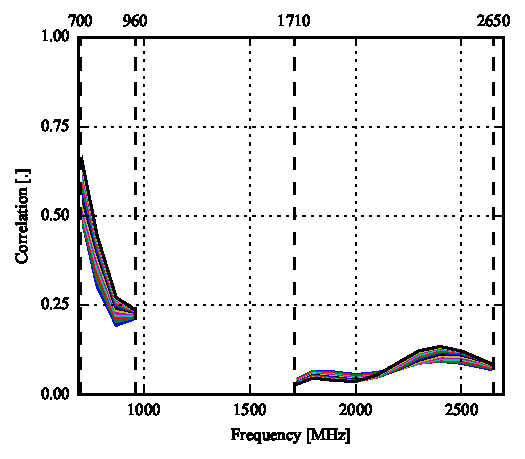
\includegraphics{img/tech_sol/trianglefeed/play_mode/correlation_Csh1-sweep}
        \caption{Sweeping $C_1$ and fixing $C_2$.}
    \end{subfigure}
    \hfill
    \begin{subfigure}{0.49\linewidth}
        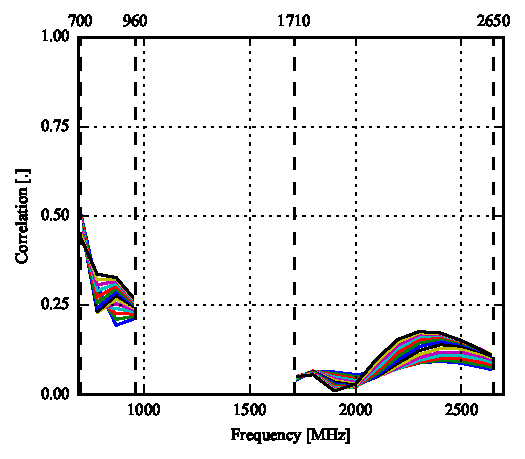
\includegraphics{img/tech_sol/trianglefeed/play_mode/correlation_Csh2-sweep}
        \caption{Sweeping $C_2$ and fixing $C_1$.}
    \end{subfigure}
    \caption{Triangle feed antenna in play mode. Correlation between antennas then sweeping tuning capacitors. Here, $C_1$ and $C_2$ are the tuning capacitor for the top and side antenna, respectively.}
    \label{fig:corr_sol2_play}
\end{figure}

% Efficiency
\begin{figure}[htbp]
    \centering
    \begin{subfigure}{0.49\linewidth}
        \centering
        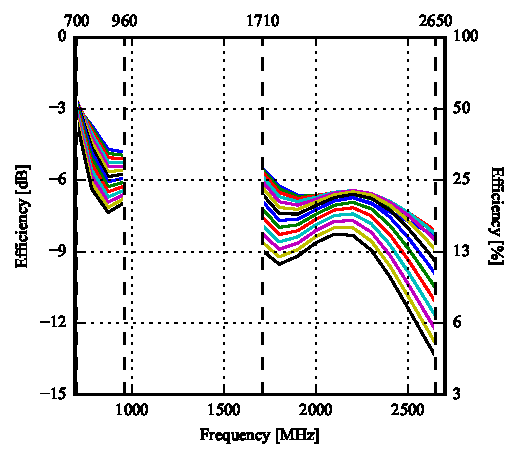
\includegraphics{img/tech_sol/trianglefeed/play_mode/efficiency-ac1-Csh1.pdf}
        \caption{Top antenna. Sweeping $C_1$, fixing $C_2$.}
    \end{subfigure}
    \hfill
    \begin{subfigure}{0.49\linewidth}
        \centering
        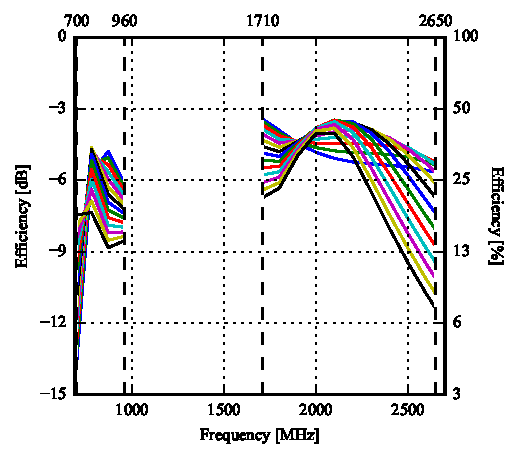
\includegraphics{img/tech_sol/trianglefeed/play_mode/efficiency-ac2-Csh2.pdf}
        \caption{Side antenna. Sweeping $C_2$, fixing $C_1$.}
    \end{subfigure}
    \caption{Triangle feed antenna in play mode. Efficiency for each antenna when sweeping the tuning capacitors. Here, $C_1$ and $C_2$ are the tuning capacitor for the top and side antenna, respectively.}
    \label{fig:eff_sol2play}
\end{figure}

\FloatBarrier
\subsection{Talk Mode}

The S-parameters with the tunable capacitors set to their minima are shown in Figure~\ref{fig:triang_sparam_talk}. The top antenna is still able to cover both the low and the high band. The side antenna's resonance, however, has been shifted down even further than in read and play mode and now only covers the very lowest part of the low band.

The S-parameters, when sweeping the tunable capacitors, are shown in Figure~\ref{fig:tiang_sparam_sweep_talk}. The maximum impedance-bandwidths are summed up in Table~\ref{tab:bw_sol2talk}. The tunable bandwidths are still large enough to cover the low-band LTE bands but the side antenna can not cover the bands up towards \SI{960}{MHz}. The high band can still be covered quite well by both antennas.

The correlation between the antennas, when sweeping the tunable capacitors, are shown in Figure~\ref{fig:corr_sol2_talk}. The correlation is very low between the antennas for every capacitor setting.

The efficiencies for each antenna, when sweeping the tuning capacitors, are shown in Figure~\ref{fig:eff_sol2talk}. In this mode, the efficiency drops very significantly. For the top antenna, the best efficiency is in the high band, peaking at around \SI{-6}{dB}. The low-band efficiency of the top antenna peaks at around \SI{-9}{dB}. The side antenna performs even worse, peaking at around \SI{-8}{dB} in the high band and at \SI{-12}{dB} in the low band. Based on this, the phone would not be very usable in talk mode. As for the SAR results, described below, the results may change when a more realistic case and screen is added to the simulation, as this might lower the influence of the users head.

\begin{figure}[htbp]
    \centering
    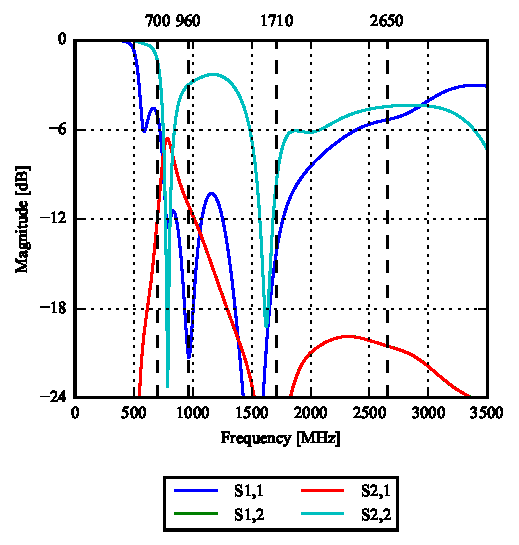
\includegraphics{img/tech_sol/trianglefeed/talk_mode/sparams.pdf}
    \caption{Triangular feed antenna in talk mode. S-parameters with both tuning capacitors fixed at \SI{0.3}{pF}.}
    \label{fig:triang_sparam_talk}
\end{figure}

\begin{table}[htbp]
    \centering
    \begin{tabular}{|l|l|r|r|r|}
        \hline
        Antenna & Band & Start [MHz] & Stop [MHz] & Bandwidth [MHz] \\
        \hline
        Top     & Low  & 701         & 2597       & 1896 \\
        Side    & Low  & 749         & 844        & 95   \\
        \hline
        Top     & High & 701         & 2597       & 1896 \\
        Side    & High & 1439        & 2516       & 1077 \\
        \hline
    \end{tabular}
    \caption{Triangle feed antenna in talk mode. Maximum bandwidth obtained in the low and high band for the top and the side antenna, respectively. It is, again, seen that both the low and high band are covered at the same time for the top antenna.}
    \label{tab:bw_sol2talk}
\end{table}

\begin{figure}[htbp]
   \begin{subfigure}[b]{0.49\linewidth}
        \centering
        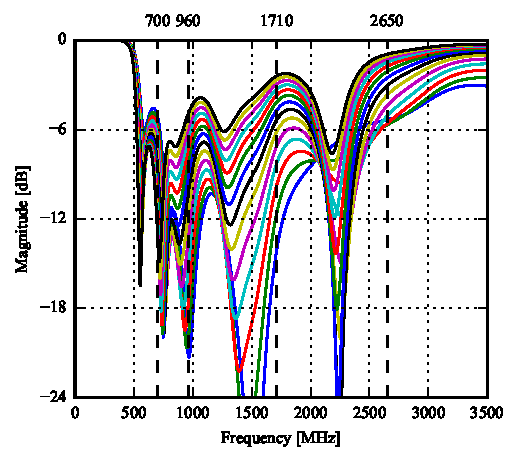
\includegraphics{img/tech_sol/trianglefeed/talk_mode/Csh1s11.pdf}
        \caption{$S_{11}$, sweeping $C_1$ and fixing $C_2$.}
    \end{subfigure}
    \hfill
    \begin{subfigure}[b]{0.49\linewidth}
        \centering
        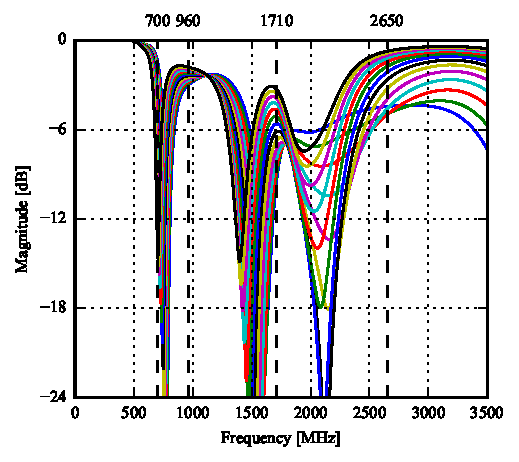
\includegraphics{img/tech_sol/trianglefeed/talk_mode/Csh2s22.pdf}
        \caption{$S_{22}$, sweeping $C_1$ and fixing $C_2$.}
    \end{subfigure}
    \\
    \begin{subfigure}[b]{0.49\linewidth}
        \centering
        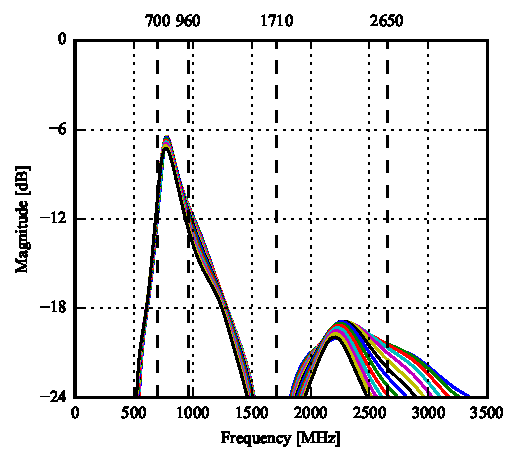
\includegraphics{img/tech_sol/trianglefeed/talk_mode/Csh1s21.pdf}
        \caption{$S_{21}$, sweeping $C_1$ and fixing $C_2$.}
    \end{subfigure}
    \hfill
    \begin{subfigure}[b]{0.49\linewidth}
        \centering
        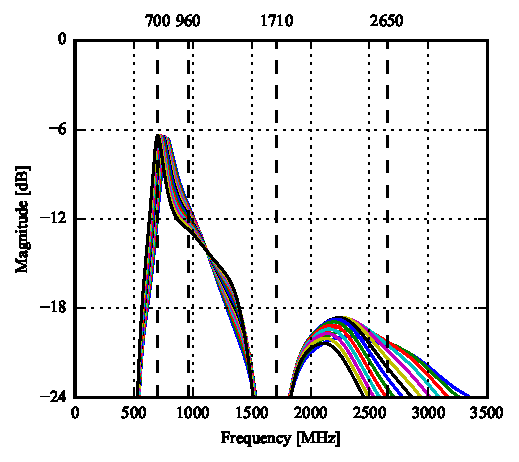
\includegraphics{img/tech_sol/trianglefeed/talk_mode/Csh2s21.pdf}
        \caption{$S_{21}$, sweeping $C_2$ and fixing $C_1$.}
    \end{subfigure}
    \caption{Triangle feed antenna in talk mode. Parameter sweep for tuning the shunt capacitor of each antenna, $C_1$ and $C_2$ for port 1 and 2, respectively. Port 1 is the top antenna and port 2 is the side antenna.}
    \label{fig:tiang_sparam_sweep_talk}
\end{figure}

% Correlation
\begin{figure}[htbp]
    \centering
    \begin{subfigure}{0.49\linewidth}
        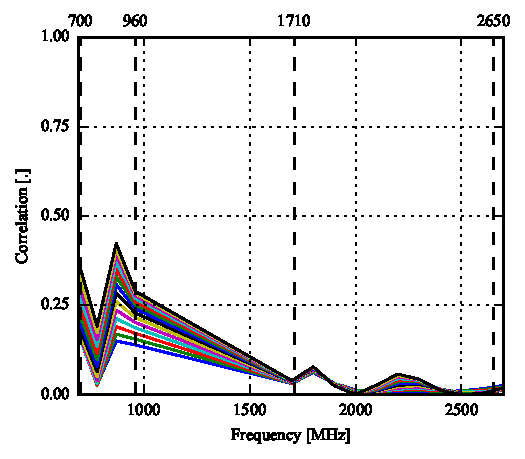
\includegraphics{img/tech_sol/trianglefeed/talk_mode/correlation_Csh1-sweep}
        \caption{Sweeping $C_1$ and fixing $C_2$.}
    \end{subfigure}
    \hfill
    \begin{subfigure}{0.49\linewidth}
        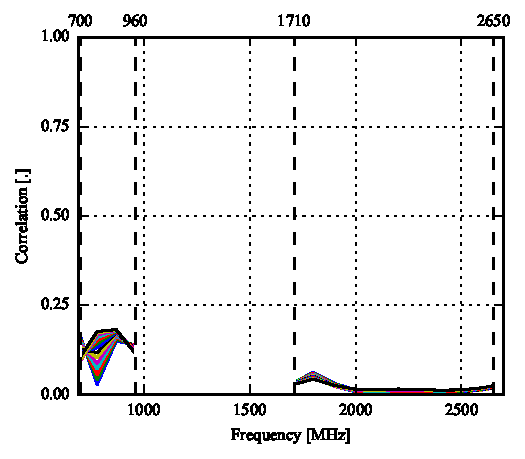
\includegraphics{img/tech_sol/trianglefeed/talk_mode/correlation_Csh2-sweep}
        \caption{Sweeping $C_2$ and fixing $C_1$.}
    \end{subfigure}
    \caption{Triangle feed antenna in talk mode. Correlation between antennas then sweeping tuning capacitors. Here, $C_1$ and $C_2$ are the tuning capacitor for the top and side antenna, respectively.}
    \label{fig:corr_sol2_talk}
\end{figure}

% Efficiency
\begin{figure}[htbp]
    \centering
    \begin{subfigure}{0.49\linewidth}
        \centering
        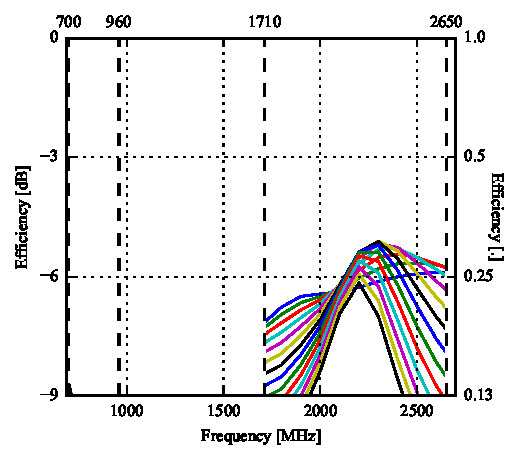
\includegraphics{img/tech_sol/trianglefeed/talk_mode/efficiency-ac1-Csh1.pdf}
        \caption{Top antenna. Sweeping $C_1$, fixing $C_2$.}
    \end{subfigure}
    \hfill
    \begin{subfigure}{0.49\linewidth}
        \centering
        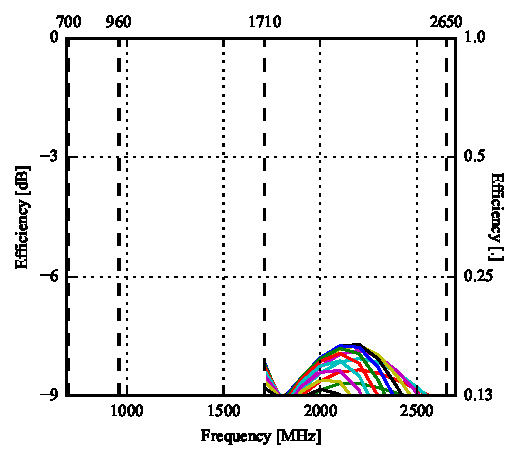
\includegraphics{img/tech_sol/trianglefeed/talk_mode/efficiency-ac2-Csh2.pdf}
        \caption{Side antenna. Sweeping $C_2$, fixing $C_1$.}
    \end{subfigure}
    \caption{Triangle feed antenna in talk mode. Efficiency for each antenna when sweeping the tuning capacitors. Here, $C_1$ and $C_2$ are the tuning capacitor for the top and side antenna, respectively.}
    \label{fig:eff_sol2talk}
\end{figure}


\FloatBarrier
\subsection{SAR}

The result from the SAR simulation is shown in Figure~\ref{fig:triang_sar_sim}. It is seen, that the maximum SAR is much larger than the required maximum of \SI{2}{W\per kg} for the side antenna. This is likely because the side antenna is very close to the head of the user as seen in Figure~\ref{fig:triang_positions}. A possible way to improve this may be to simulate the phone's screen, which will be located between (part of) the antenna and the head. This may reflect some of the radiated power away from the user, lowering the maximum SAR.

To fulfill the SAR requirements, it is possible to only one the top antenna for the uplink, where most power is emitted, and use both antennas in the downlink. For this reason, no further SAR simulations are performed at this point.

\begin{figure}[htbp]
    \centering
    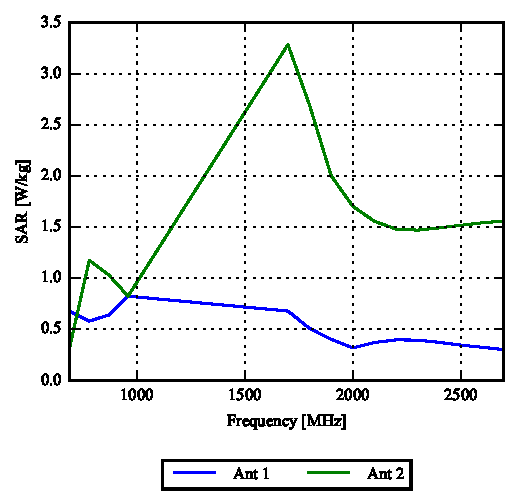
\includegraphics{img/tech_sol/trianglefeed/sar/sar.pdf}
    \caption{SAR simulation of the triangle feed antenna.}
    \label{fig:triang_sar_sim}
\end{figure}

\fixme{Re-do simulations with more realistic cover?}

